\chapter{Optimization}



The foundation of engineering is the ability to use math and physics to design and optimize complex systems.
The advent of computers has made this possible on an unprecedented scale.
This chapter provides a brief introduction to mathematical optimization theory.

\section{Derivatives in Banach Spaces}

In this chapter, we assume that readers are familiar with derivatives as defined in undergraduate multivariable calculus.
To gain insight, we first recall the standard interpretation of the derivative as a local linear approximation of a function.
For a function $f\colon \RealNumbers^n \to \RealNumbers^m$, this interpretation gives 
\[ f(\vecnot{x} + \vecnot{h}) = f(\vecnot{x}) + J(\vecnot{x}) \cdot \vecnot{h} + \text{higher order terms}, \]
where $J(\vecnot{x})\in \RealNumbers^{m\times n}$ is the Jacobian matrix of $f$ at $\vecnot{x}$.

Instead of interpreting a multivariate derivative as a matrix,  we will view the derivative $f'(x)$ as a linear transform $T$ from the domain to codomain.
This transform maps the input perturbation $\vecnot{h}$ to a local approximation of the output perturbation.
Since both are finite dimensional in our example, the linear transform $T$ is represented by the Jacobian matrix and we have $$f'(\vecnot{x})(\vecnot{h}) = T \vecnot{h} = J(\vecnot{x})\cdot \vecnot{h}.$$ 

Mathematically, such definitions require the structure of a Banach space because one needs the linear structure to compute differences, the norm topology to define limits, and completeness to guarantee that the limits exists under mild conditions.

\begin{definition}
Let $f \colon X \rightarrow Y$ be a mapping from a vector space $X$ over $\RealNumbers$ to a Banach space $(Y,\|\cdot\|)$.
Then, if it exists, the \defn{optimization}{G\^{a}teaux differential} (or directional derivative) of $f$ at $\vecnot{x}$ in direction $\vecnot{h}$ is given by
\[ \delta f (\vecnot{x};\vecnot{h}) \triangleq \lim_{t \to 0} \frac{f(\vecnot{x}+t \vecnot{h}) - f(\vecnot{x})}{t}, \]
where the limit is with respect to the implied mapping from $t\in \RealNumbers$ to $Y$.
%convergence is defined with respect to the norm of $Y$.
\end{definition}

\begin{lemma}
\label{lemma:gateaux_negative}
Let $Y = (\RealNumbers,|\cdot|)$ and suppose that $\delta f (\vecnot{x};\vecnot{h})$ exists and is negative for some $f$, $\vecnot{x}$, and $\vecnot{h}$.  Then, there exists $t_0 > 0$ such that, for all $t\in(0,t_0)$, one has
\[ f(\vecnot{x}+t \vecnot{h}) < f (\vecnot{x}). \]
\end{lemma}
\begin{proof}
The $\delta f (\vecnot{x};\vecnot{h})$ limit implies that, for any $\epsilon > 0$, there is a $t_0 > 0$ such that
\[ f(\vecnot{x}+t \vecnot{h}) - f (\vecnot{x}) \leq \left( \delta f (\vecnot{x};\vecnot{h}) + \epsilon \right)t \]
for all $t\in (0,t_0)$.
If $\delta f (\vecnot{x};\vecnot{h})<0$, then one can choose $\epsilon = -\frac{1}{2}\delta f (\vecnot{x};\vecnot{h})$ to see that the RHS is negative for all $t\in (0,t_0)$.
The stated result follows.
\end{proof}

\begin{example}
For the standard Banach space $X\!=\!Y\!=\!\mathbb{R}^2$, let $f(\vecnot{x})\! =\! (x_1 x_2,x_1+x_2^2)$.
Then, for $\vecnot{x}\!=\!(1,1)$, $\vecnot{h}\!=\!(1,2)$, we have
\[ \delta f ( \vecnot{x},\vecnot{h} ) = \frac{d}{dt} ((1+t)(1+2t),(1+t)+(1+2t)^2) \Big|_{t=0} = (3,5). \]
\end{example}

\begin{problem}
Suppose $X=Y=L^1 ([0,1])$ is the Banach space of Lebesgue absolutely integrable functions mapping $[0,1]$ to $\RealNumbers$ and $f(\vecnot{x}) = \| \vecnot{x} \| = \int_0^1 |x(s)| \dd s$ is the norm of $\vecnot{x}$.
Assuming the set $\{ s\in [0,1] | x(s)=0 \}$ has measure 0, show that
\[ \delta f (\vecnot{x};\vecnot{h}) \triangleq \lim_{t \to 0}  \int_0^1 \frac{1}{t} \left( |x(s)+t h(s)| - |x(s)| \right) \dd s = \int_0^1 \mathrm{sgn}(x(s)) h(s) \dd s. \] 
\end{problem}

\begin{definition}
Let $f \colon X \rightarrow Y$ be a mapping from a vector space $X$ over $\RealNumbers$ to a Banach space $(Y,\|\cdot\|)$.
Then, $f$ is \defn{optimization}{G\^{a}teaux differentiable} at $\vecnot{x}$ if the G\^{a}teaux differential $\delta f (\vecnot{x};\vecnot{h})$ exists for all $\vecnot{h} \in X$ and is a linear function of $\vecnot{h}$.
If, in addition, $X$ is a Banach space, then $\delta f (\vecnot{x};\vecnot{h})$ must be a continuous linear function of $\vecnot{h}$.
\end{definition}

\begin{remark}
For simplicity, our treatment of G\^{a}teaux derivatives assumes $X$ is a vector space over $\RealNumbers$ but similar results are possible over $\ComplexNumbers$ as well.
\end{remark}

\begin{definition}
Let $f \colon X \rightarrow Y$ be a mapping from a Banach space $(X,\|\cdot\|_X)$ to a Banach space $(Y,\|\cdot\|_Y)$.
Then, $f$ is \defn{optimization}{Fr\'{e}chet differentiable} at $\vecnot{x}$ if there is a linear transformation $T\colon X \to Y$ with $\| T \| < \infty$ that satisfies 
\begin{equation} \label{eq:frechet_def}
\lim_{\vecnot{h} \to \vecnot{0}} \frac{\left\|f(\vecnot{x}+ \vecnot{h}) - f(\vecnot{x}) - T(\vecnot{h}) \right\|_Y}{\| \vecnot{h} \|_X} = 0,
\end{equation}
where the limit is with respect to the implied Banach space mapping $X\to \RealNumbers$.
In this case, the \defn{optimization}{Fr\'{e}chet derivative} at $\vecnot{x}$ equals $T$ and is denoted by $f'(\vecnot{x})$ in general.
\end{definition}

\begin{example}
A function $f\colon \RealNumbers^n \to \RealNumbers^m$ with $f = (f_1,f_2,\ldots,f_m)^T$ is (Fr\'{e}chet) differentiable at $\vecnot{x}_0$ if the mapping $J$ from $\RealNumbers^n$ to the \defn{optimization}{Jacobian matrix},
\[ J(\vecnot{x})=f'(\vecnot{x}) \triangleq \left[ \begin{array}{cccc} \frac{\partial  f_1}{\partial  x_1} (\vecnot{x}) & \frac{\partial  f_1}{\partial  x_2} (\vecnot{x}) & \cdots & \frac{\partial  f_1}{\partial  x_n} (\vecnot{x}) \\
\frac{\partial  f_2}{\partial  x_1} (\vecnot{x}) & \frac{\partial  f_2}{\partial  x_2} (\vecnot{x}) & \cdots & \frac{\partial  f_2}{\partial  x_n} (\vecnot{x}) \\
\vdots & \vdots & \ddots & \vdots \\
\frac{\partial  f_m}{\partial  x_1} (\vecnot{x}) & \frac{\partial  f_m}{\partial  x_2} (\vecnot{x}) & \cdots & \frac{\partial  f_m}{\partial  x_n} (\vecnot{x}) \end{array} \right], \]
exists and is continuous in $\vecnot{x}$ at $\vecnot{x}=\vecnot{x}_0$.
A necessary and sufficient condition for this is that each partial derivative is continuous in $\vecnot{x}$ at $\vecnot{x}=\vecnot{x}_0$.

If $m=1$, then the Jacobian is also called the \defn{optimization}{gradient} of the function
\[ f'(\vecnot{x}) = \nabla f(\vecnot{x}) \triangleq \left[ \begin{array}{cccc} \frac{\partial  f}{\partial  x_1} (\vecnot{x}) & \frac{\partial  f}{\partial  x_2} (\vecnot{x}) & \cdots & \frac{\partial  f}{\partial  x_n} (\vecnot{x}) \end{array} \right]. \]
It is worth noting that there is no universal agreement about the orientation of the gradient vector (i.e., row versus column vector).
This is because derivatives are properly understood as linear transforms and either orientation can be used to define the correct linear transform. 
\end{example}

\begin{example}
Let $X$ be a Hilbert space over $\RealNumbers$ and $f\colon X \to \RealNumbers$ be a real functional.
If the Fr\'{e}chet derivative $f'(\vecnot{x})$ exists, then it is a continuous linear functional on $X$.
Thus, the Riesz representation theorem guarantees that there is a vector $\vecnot{u} \in X$ such that
$ f'(\vecnot{x})(\vecnot{h}) = \langle\vecnot{h} | \vecnot{u} \rangle $ for all $\vecnot{h}\in X$.
This vector is called the gradient $\nabla f(\vecnot{x})$ and it follows that
$$ f'(\vecnot{x})(\vecnot{h}) = \langle\vecnot{h} | \nabla f (\vecnot{x}) \rangle \text{ for all } \vecnot{h}\in X. $$
\end{example}

\begin{problem}
In the setting of the previous example, show that, if $\nabla f (\vecnot{x}) \neq \vecnot{0}$, then $f\big(\vecnot{x}-\delta \nabla f(\vecnot{x})\big) < f(\vecnot{x})$ for some $\delta >0$.
\end{problem}

\begin{theorem} \label{theorem:frechet2gateaux}
Let $f \colon X \rightarrow Y$ be a mapping from a Banach space $(X,\|\cdot\|_X)$ to a Banach space $(Y,\|\cdot\|_Y)$.
If $f$ is Fr\'{e}chet differentiable at $\vecnot{x}$ with derivative $f'$, then $f$ is G\^{a}teaux differentiable at $\vecnot{x}$ with G\^{a}teaux differential $\delta f (\vecnot{x};\vecnot{h}) = f'(\vecnot{x}) (\vecnot{h})$.
\end{theorem}
\begin{proof}
For $\vecnot{h} = \vecnot{0}$, the statement is trivial.
For $\vecnot{h} \neq \vecnot{0}$, we first observe that $t\vecnot{h} \to \vecnot{0}$ as $t \to 0$.
Letting $T=f'(\vecnot{x})$, we can combine this with~\eqref{eq:frechet_def} to see that
\begin{align*}
0 &= \lim_{t \to 0} \frac{\left\|f(\vecnot{x}+ t\vecnot{h}) - f(\vecnot{x}) - T(t\vecnot{h}) \right\|_Y}{\| t\vecnot{h} \|_X} \\
&= \lim_{t \to 0} \left\|\frac{f(\vecnot{x}+ t\vecnot{h}) - f(\vecnot{x})}{t \| \vecnot{h} \|_X} - \frac{ t T(\vecnot{h})}{t \| \vecnot{h} \|_X} \right\|_Y \\
&= \frac{1}{\| \vecnot{h} \|_X}  \lim_{t \to 0} \left\|\frac{f(\vecnot{x}+ t\vecnot{h}) - f(\vecnot{x})}{t} - T(\vecnot{h}) \right\|_Y.
\end{align*}
Thus, the G\^{a}teaux differential exists and satisfies $\delta f (\vecnot{x};\vecnot{h}) = T (\vecnot{h}) = f'(\vecnot{x}) (\vecnot{h})$.
\end{proof}

\begin{theorem}
Let $X,Y,Z$ be Banach spaces and let $f \colon X \rightarrow Y$ and $g\colon Y \to Z$ be functions.
If $f$ is Fr\'{e}chet differentiable at $\vecnot{x}$ and $g$ is Fr\'{e}chet differentiable at $\vecnot{y}=f(\vecnot{x})$, then $(g \circ f) (\vecnot{x}) = g(f(\vecnot{x}))$ is Fr\'{e}chet differentiable at $\vecnot{x}$ with derivative $g'(f(\vecnot{x}))\circ f'(\vecnot{x})$.
\end{theorem}

\begin{proof}
For the stated derivatives, the errors in the implied linear approximations are 
\begin{align*}
\phi(\vecnot{v}) &= f(\vecnot{x} + \vecnot{v})-f(\vecnot{x}) - f'(\vecnot{x})(\vecnot{v}) \\
\psi(\vecnot{u}) &= g(\vecnot{y} + \vecnot{u})-g(\vecnot{y}) - g'(\vecnot{y})(\vecnot{u}) \\
\rho(\vecnot{h}) &= g(f(\vecnot{x} + \vecnot{h})) -g(f(\vecnot{x})) - \left( g'(\vecnot{y}) \circ f'(\vecnot{x})\right) (\vecnot{h}).
\end{align*}
From the assumptions of differentiability, we know that the first two approximations become tight for small perturbations.
In other words,
\begin{align*}
\lim_{\vecnot{v} \to \vecnot{0}} \frac{\| \phi (\vecnot{v}) \|_Y}{\|\vecnot{v}\|_X} = 0,  \quad\quad\quad\quad \lim_{\vecnot{u} \to \vecnot{0}} & \frac{\| \psi (\vecnot{u})\|_Z}{\|\vecnot{u}\|_Y} = 0.
\end{align*}
Next, we observe that the definition of $\phi$ implies
\[ g(f(\vecnot{x} + \vecnot{h})) -g(f(\vecnot{x})) = g \big( f(\vecnot{x}) + f'(\vecnot{x})(\vecnot{h}) + \phi(\vecnot{h}) \big) - g(\vecnot{y}). \]
Combining this with the definition of $\rho$ shows that
\begin{align*}
\rho(\vecnot{h}) &= g \big( f(\vecnot{x}) + f'(\vecnot{x})(\vecnot{h}) + \phi(\vecnot{h}) \big) - g(\vecnot{y}) - \left( g'(\vecnot{y}) \circ f'(\vecnot{x})\right) (\vecnot{h}) \\
&= \psi \big(f'(\vecnot{x})(\vecnot{h}) + \phi(\vecnot{h}) \big) + g'(\vecnot{y})\big( f'(\vecnot{x})(\vecnot{h}) + \phi(\vecnot{h}) \big) - \left( g'(\vecnot{y}) \circ f'(\vecnot{x})\right) (\vecnot{h}) \\
&= \psi \big(f'(\vecnot{x})(\vecnot{h}) + \phi(\vecnot{h}) \big) + g'(\vecnot{y})(\phi(\vecnot{h})).
\end{align*}
We take this opportunity to note that $\|g'(f(\vecnot{x}))\circ f'(\vecnot{x})\| \leq \|g'(f(\vecnot{x}))\| \|f'(\vecnot{x})\| \leq \infty$ because $\|f'(\vecnot{x})\|\leq \infty$ and $\|g'(f(\vecnot{x}))\| <\infty$. 
Since $\lim_{\vecnot{h} \to \vecnot{0}} \| \phi (\vecnot{h}) \|_Y / \|\vecnot{h}\|_X = 0$, there is a $t>0$ such that $\|\phi(\vecnot{h})\|_Y \leq \|f'(\vecnot{x})\| \|\vecnot{h}\|_X$ if $\|\vecnot{h}\|_X < t$.
Under the same condition, it follows that $2 \|f'(\vecnot{x})\| \|\vecnot{h}\|_X \geq \|f'(\vecnot{x})\| \|\vecnot{h}\|_X + \| \phi(\vecnot{h}) \|_Y$. 
Using this, we can write
\begin{align*}
\frac{\|\rho(\vecnot{h})\|_Z}{\|\vecnot{h}\|_X}
&= \frac{\| \psi \big(f'(\vecnot{x})(\vecnot{h}) + \phi(\vecnot{h}) \big) + g'(\vecnot{y})(\phi(\vecnot{h})) \|_Z}{\|\vecnot{h}\|_X} \\
&\leq 2 \|f'(\vecnot{x})\|  \frac{\| \psi \big(f'(\vecnot{x})(\vecnot{h}) + \phi(\vecnot{h}) \big) \|_Z}{ 2 \|f'(\vecnot{x})\|  \|\vecnot{h}\|_X} + \frac{\|  g'(\vecnot{y})(\phi(\vecnot{h})) \|_Z}{\|\vecnot{h}\|_X} \\
& \leq 2 \|f'(\vecnot{x})\| \frac{\| \psi \big(f'(\vecnot{x})(\vecnot{h}) + \phi(\vecnot{h}) \big) \|_Z}{\|f'(\vecnot{x})\| \|\vecnot{h}\|_X + \| \phi(\vecnot{h}) \|_Y} + \frac{\|  g'(\vecnot{y})\| \|\phi(\vecnot{h}) \|_Y}{\|\vecnot{h}\|_X} \\
& \leq 2 \|f'(\vecnot{x})\| \frac{\| \psi \big(f'(\vecnot{x})(\vecnot{h}) + \phi(\vecnot{h}) \big) \|_Z}{\|f'(\vecnot{x}) (\vecnot{h}) + \phi(\vecnot{h})\|_Y} + \frac{\|  g'(\vecnot{y})\| \|\phi(\vecnot{h}) \|_Y}{\|\vecnot{h}\|_X}.
\end{align*}
Since $(f'(\vecnot{x}) (\vecnot{h}) + \phi(\vecnot{h})) \to \vecnot{0}$ as $\vecnot{h}\to\vecnot{0}$, it follows that the limit of the RHS, as $\vecnot{h}\to\vecnot{0}$, also exists and equals 0.
Thus, $\lim_{\vecnot{h} \to \vecnot{0}} \| \rho (\vecnot{h}) \|_Z / \|\vecnot{h}\|_X = 0$ and the Fr\'{e}chet derivative of $g(f(\vecnot{x}))$ exists and satisfies the chain rule.
\end{proof}

%\iffalse
\begin{theorem} \label{theorem:mean_value_inequality}
Let $X,Y$ be Banach spaces and $f \colon X \rightarrow Y$ be a function.
For $\vecnot{x}_1,\vecnot{x}_2 \in X$, let $\vecnot{h} = \vecnot{x}_2 - \vecnot{x}_1$ and assume the G\^{a}teaux differential $\delta f \big( (1-s)\vecnot{x}_1+s\vecnot{x}_2; \vecnot{h}\big)$ exists for all $s\in [0,1]$.
Then, $\|f(\vecnot{x}_2)-f(\vecnot{x}_1)\| \leq M \| \vecnot{x}_2 - \vecnot{x}_1 \|$, where
\[ M = \frac{\sup_{s \in [0,1]} \| \delta f \big( (1-s)\vecnot{x}_1+s\vecnot{x}_2; \vecnot{h}\big)\|}{\| \vecnot{x}_2 - \vecnot{x}_1 \|}. \]
\end{theorem}
\begin{proof}
For $\vecnot{w}_1 = \frac{1}{2}(\vecnot{x}_1+\vecnot{x}_2)$, observe that
\begin{align*}
\frac{\|f(\vecnot{x}_2)-f(\vecnot{x}_1)\|}{\| \vecnot{x}_2 - \vecnot{x}_1 \|} &=  \frac{\|f(\vecnot{x_2})-f(\vecnot{w}_1) + f(\vecnot{w}_1)-f(\vecnot{x}_1)\|}{\| \vecnot{x}_2 - \vecnot{x}_1 \|} \\
&\leq 
 \frac{\|f(\vecnot{x}_2)-f(\vecnot{w}_1)\| + \|f(\vecnot{w}_1)-f(\vecnot{x}_1)\|}{\| \vecnot{x}_2 - \vecnot{x}_1 \|} \\
&=  \frac{\|f(\vecnot{x}_2)-f(\vecnot{w}_1)\|}{2 \| \vecnot{x}_2 - \vecnot{w}_1 \|} +  \frac{\|f(\vecnot{w}_1)-f(\vecnot{x}_1)\|}{2 \| \vecnot{w}_1 - \vecnot{x}_1 \|}.
\end{align*}
Suppose that $\|f(\vecnot{x}_2)-f(\vecnot{x}_1)\| > M \| \vecnot{x}_2 - \vecnot{x}_1\|$.
Then, there is an $\epsilon > 0$ such that one or both of the following conditions must hold:
\[ \frac{\|f(\vecnot{x}_2)-f(\vecnot{w}_1)\|}{\| \vecnot{x}_2 - \vecnot{w}_1 \|} \geq M + \epsilon  \quad \text{and} \quad \frac{\|f(\vecnot{w}_1)-f(\vecnot{x}_1)\|}{\| \vecnot{w}_1 - \vecnot{x}_1 \|} \geq M + \epsilon. \]
Repeating indefinitely and choosing a satisfying subinterval at each step, one gets a sequence $\vecnot{w}_n$ of midpoints that converges to $\vecnot{x}=  (1-s)\vecnot{x}_1+s\vecnot{x}_2 $ for some $s\in [0,1]$.
Since the G\^{a}teaux differential $\delta f (\vecnot{x};\vecnot{h})$ exists by assumption, it follows that
\[ M + \epsilon \leq \frac{\|f(\vecnot{w}_n)-f(\vecnot{x})\|}{\| \vecnot{w}_n - \vecnot{x} \|} = \left\| \frac{f(\vecnot{x}\pm 2^{-n} \vecnot{h})-f(\vecnot{x})}{2^n \| \vecnot{x}_2 - \vecnot{x}_1 \|} \right\| \to \frac{\| \delta f (\vecnot{x};\vecnot{h}) \|}{\| \vecnot{x}_2 - \vecnot{x}_1 \|}. \] 
This contradicts the definition of $M$ and, thus, $\|f(\vecnot{x}_2)-f(\vecnot{x}_1)\| \leq M \| \vecnot{x}_2 - \vecnot{x}_1\|$.
\end{proof}

\begin{corollary}
Let $X,Y$ be Banach spaces and $f \colon X \rightarrow Y$ be a function.
If the Fr\'{e}chet derivative $f'(\vecnot{x})$ exists and satisfies $\| f'(\vecnot{x})\| \leq L$ for all $\vecnot{x}$ in a convex set $A\subseteq X$, then $f$ is Lipschitz continuous on $A$ with Lipschitz constant $L$.
\end{corollary}

\begin{proof}
Assume $\| f'(\vecnot{x})\| \leq L$ for all $\vecnot{x}$ in a convex set $A\subseteq X$.
Then, for any $\vecnot{x}_1 , \vecnot{x}_2 \in A$, let $\vecnot{h} = \vecnot{x}_2 - \vecnot{x}_1$ and notice that Theorem~\ref{theorem:frechet2gateaux} implies that
\[ \| \delta f \big( (1-s)\vecnot{x}_1+s\vecnot{x}_2; \vecnot{h}\big) \|  = \| f'\big( (1-s)\vecnot{x}_1+s\vecnot{x}_2 \big)(\vecnot{h}) \| \leq \| f'(\vecnot{x})\| \|\vecnot{h} \|, \] 
for all $s\in [0,1]$.
Applying Theorem~\ref{theorem:mean_value_inequality}, we see that $\|f(\vecnot{x}_2)-f(\vecnot{x}_1)\| \leq M \| \vecnot{x}_2 - \vecnot{x}_1\|$ with $M \leq \| f'(\vecnot{x})\| \leq L$.
This completes the proof.
\end{proof}
%\fi

\iffalse
\begin{theorem}
Let $f\colon \RealNumbers^n \to \RealNumbers^m$ defined by $f = (f_1,f_2,\ldots,f_m)^T$ where $f_i \colon \RealNumbers^n \to \RealNumbers$ are real functions.
In this problem, the sets $\RealNumbers^n$, $\RealNumbers^m$, and $\RealNumbers$ are treated as Banach spaces with norms
$\|\vecnot{x} \| \triangleq \sum_{i=1}^d |x_i|$, where $d$ is the dimension.
If $\frac{\partial f_i}{\partial x_j} (\vecnot{x})$ exists and is continuous in $\vecnot{x}$, then the mapping $f$ is Fr\'{e}chet differentiable  at $\vecnot{x}$.
\end{theorem}
\begin{proof}
For $\vecnot{h} \in \RealNumbers^n$, let $\phi_j (\vecnot{h}) \triangleq (h_1,h_2,\ldots,h_j,0,\ldots,0)$ and observe that
\[ f(\vecnot{x}+\vecnot{h}) - f(\vecnot{x}) = \sum_{j=1}^n f(\vecnot{x}+\phi_j (\vecnot{h})) - f(\vecnot{x}+\phi_{j-1}(\vecnot{h})). \]
Also, the existence of $\frac{\partial f_i}{\partial x_j} (\vecnot{x})$ implies that, for any $\epsilon >0$, there is a $\delta_j > 0$ such that
\[  \left| \left[ f(\vecnot{x}+\phi_j (\vecnot{h})) - f(\vecnot{x}+\phi_{j-1}(\vecnot{h})) \right]_i  - h_j \frac{\partial f_i}{\partial x_j} (\vecnot{x}+\phi_{j-1}(\vecnot{h})) \right| < \frac{\epsilon}{n} |h_j| \]
for all $|h_j| < \delta_j$.
Using this to bound the norm of the implied sum, we see that
\[  \left\| f(\vecnot{x}+\phi_j (\vecnot{h})) - f(\vecnot{x}+\phi_{j-1}(\vecnot{h})) -  h_j \sum_{i=1}^m \vecnot{e}_i \frac{\partial f_i}{\partial x_j}  (\vecnot{x}+\phi_{j-1}(\vecnot{h})) \right\|  < \epsilon |h_j| \]
for all $|h_j| < \delta_j$.
Now, let us define
\[ g(\vecnot{x})(\vecnot{h}) = \sum_{j=1}^n h_j \sum_{i=1}^m \vecnot{e}_i \frac{\partial f_i}{\partial x_j} (\vecnot{x}+\phi_{j-1}(\vecnot{h})) \]
and observe that
\begin{align*}
\| f(\vecnot{x}+\vecnot{h}) & - f(\vecnot{x}) - g(\vecnot{x}) (\vecnot{h}) \|  \\
&\leq \sum_{j=1}^n \left\| f(\vecnot{x}+\phi_j (\vecnot{h})) - f(\vecnot{x}+\phi_{j-1}(\vecnot{h})) - h_j \sum_{i=1}^m \vecnot{e}_i \frac{\partial f_i}{\partial x_j} (\vecnot{x}+\phi_{j-1}(\vecnot{h})) \right\| \\
& \leq \sum_{j=1}^n \sum_{i=1}^m \epsilon |h_j| = \epsilon \| \vecnot{h} \|.
\end{align*}
Next, we note that
\begin{align*}
\| g(\vecnot{x})(\vecnot{h}) &- f'(\vecnot{x})(\vecnot{h}) \| \\
&= \left\| \sum_{j=1}^n h_j \sum_{i=1}^m \vecnot{e}_i \frac{\partial f_i}{\partial x_j} (\vecnot{x}+\phi_{j-1}(\vecnot{h})) - \sum_{j=1}^n h_j \sum_{i=1}^m \vecnot{e}_i \frac{\partial f_i}{\partial x_j} (\vecnot{x}) \right\| \\
&\leq \sum_{j=1}^m |h_j| \sum_{i=1}^m \left| \frac{\partial f_i}{\partial x_j} (\vecnot{x}+\phi_{j-1}(\vecnot{h})) - \frac{\partial f_i}{\partial x_j} (\vecnot{x}) \right|.
\end{align*}
Since each $\frac{\partial f_i}{\partial x_j} (\vecnot{x})$ is continuous, for any $\epsilon>0$, there is a $\delta_{i,j}>0$ such that
\[ \left| \frac{\partial f_i}{\partial x_j} (\vecnot{x}+\phi_{j-1}(\vecnot{h})) - \frac{\partial f_i}{\partial x_j} (\vecnot{x}) \right| < \frac{\epsilon}{n} \]
for all $|h_j| < \delta_{i,j}$.
Then, it follows that
\begin{align*}
\| f(\vecnot{x}+\vecnot{h}) & - f(\vecnot{x}) - f'(\vecnot{x}) (\vecnot{h}) \|  \\ &\leq \| f(\vecnot{x}+\vecnot{h}) - f(\vecnot{x}) - g(\vecnot{x}) (\vecnot{h}) \| + \| g(\vecnot{x})(\vecnot{h}) - f'(\vecnot{x}) (\vecnot{h}) \| \\
&\leq \epsilon \|\vecnot{h}\| + \sum_{j=1}^m |h_j| \sum_{i=1}^m \left| \frac{\partial f_i}{\partial x_j} (\vecnot{x}+\phi_{j-1}(\vecnot{h})) - \frac{\partial f_i}{\partial x_j} (\vecnot{x}) \right| \\
&\leq  2 \epsilon \| \vecnot{h} \| 
\end{align*}
for all $\| \vecnot{h} \| < \delta$ where $\delta$ the minimum of all previous $\delta$'s.
Thus, we can divide both sides by $\|\vecnot{h}\|$ to show the limit in~\eqref{eq:frechet_def} exists and $f(\vecnot{x})$ is Fr\'{e}chet differentiable.
\end{proof}
\fi


\section{Unconstrained Optimization}

Functions mapping elements of a vector space (over $F$) down to the scalar field $F$ play a very special role in the analysis of vector spaces.

\begin{definition}
Let $V$ be a vector space over $F$.
Then, a \defn{vector space}{functional} on $V$ is a function $f \colon V \rightarrow F$ that maps $V$ to $F$.
\end{definition}

Linear functionals (i.e., functionals that are linear) are used to define many important concepts in abstract vector spaces.
For unconstrained optimization, however, linear functionals are not interesting because they are either zero or they achieve all values in $F$.
%Instead, this section focuses on non-linear functionals.

\begin{definition}
\label{definition:minimum_value}
Let $(X,\|\cdot\|)$ be a normed vector space.
Then, a real functional $f \colon X \rightarrow \RealNumbers$ achieves a \defn{optimization}{local minimum value} at $\vecnot{x}_0 \in X$ if there is an $\epsilon > 0$ such that, for all $\vecnot{x}\in X$ satisfying $\| \vecnot{x} - \vecnot{x}_0 \| < \epsilon$, we have  $f(\vecnot{x}) \geq f(\vecnot{x}_0)$.
If the bound holds for all $x\in X$, then the local minimum is also a \defn{functions}{global minimum value}.
\end{definition}

\begin{theorem}
Let $(X,\|\cdot\|)$ be a normed vector space and $f\colon X \to \mathbb{R}$ be a real functional.
If $\delta f (\vecnot{x}_0,\vecnot{h})$ exists and is negative for any $\vecnot{h} \in X$, then $\vecnot{x}_0$ is not a local minimum value.
\end{theorem}
\begin{proof}
First, we apply Lemma~\ref{lemma:gateaux_negative} with the $\vecnot{x}$ and $\vecnot{h}$ for which $\delta f (\vecnot{x}_0,\vecnot{h})<0$.
This gives a $t_0 >0$ such that $f(\vecnot{x}_0+t \vecnot{h})<f(\vecnot{x}_0)$ for all $t\in (0,t_0)$.
Thus, there can no be no $\epsilon>0$ satisfying the definition of a local minimum value in  Definition~\ref{definition:minimum_value}.
\end{proof}

\section{Convex Functionals}

Convexity is a particularly nice property of spaces and functionals that leads to well-defined minimum values.




\begin{definition}
Let $V$ be a vector space, $A \subseteq V$ be a convex set, and $f \colon V \rightarrow \RealNumbers$ be a functional.
Then, a functional $f$ is called \defn{functions}{convex} on $A$ if, for all $\vecnot{a}_1,\vecnot{a}_2 \in A$ and $\lambda\in(0,1)$, we have
\[ f( \lambda \vecnot{a}_1 + (1-\lambda) \vecnot{a}_2 ) \leq \lambda f( \vecnot{a}_1 ) + (1-\lambda) f ( \vecnot{a}_2 ). \]
The functional is \textbf{strictly convex} if equality occurs only when $\vecnot{a}_1 = \vecnot{a}_2$.
A functional is $f$ is called (strictly) \defn{functions}{concave} if $-f$ is (strictly) convex.
\end{definition}

\begin{definition}
A Banach space $X$ is called \defn{Banach space}{strictly convex} if the unit ball,  given by $\{ x\in X | \, \| x \| \leq 1 \}$, is a strictly convex set.
An equivalent condition is that equality in the triangle inequality (i.e., $\| \vecnot{x} + \vecnot{y} \| = \| \vecnot{x} \| + \| \vecnot{y} \|$) for non-zero vectors implies that $ \vecnot{x} = s \vecnot{y} $ for some $s\in F$.
\end{definition}

\begin{example}
Let $(X,\|\cdot\|)$ be a normed vector space.
Then, the norm $\| \cdot \| \colon X \rightarrow \mathbb{R}$ is a convex functional on $X$.
Proving this is a good introductory exercise.
\end{example}

\begin{example}
Let $X$ be an an inner-product space. For $\vecnot{x},\vecnot{y} \in X$ and $\lambda \in (0,1)$,
\begin{align*}
\|\lambda \vecnot x + (1-\lambda) \vecnot y \|^2
&= \lambda^2 \| \vecnot x\|^2 + 2\lambda(1-\lambda) \Real \langle \vecnot x |  \vecnot y \rangle + (1-\lambda)^2 \|\vecnot y\|^2 \\
&= \lambda \| \vecnot x\|^2 + (1-\lambda)\|\vecnot y\|^2 - \lambda (1-\lambda) (\|\vecnot x\|^2+\|\vecnot y\|^2-2 \Real \langle x | y \rangle)\\
&= \lambda \| \vecnot x\|^2 + (1-\lambda)\|\vecnot y\|^2 - \lambda (1-\lambda) \|\vecnot x - \vecnot y\|^2 \\
&\leq \lambda \| \vecnot x\|^2 + (1-\lambda)\|\vecnot y\|^2,
\end{align*}
with equality iff $\vecnot{x}=\vecnot{y}$.
Thus, the square of the induced norm $\| \cdot \|^2$ is a strictly convex functional on $X$.
\end{example}

\begin{theorem}
\label{theorem:convex_unique_min}
Let $(X,\|\cdot\|)$ be a normed vector space, $A \subseteq X$ be a convex set, and $f \colon X \rightarrow \RealNumbers$ be a convex functional on $A$.
Then, any local minimum value of $f$ on $A$ is a global minimum value on $A$.
If the functional is strictly convex on $A$ and achieves a local minimum value on $A$, then there is a unique point $\vecnot{x}_0 \in A$ that achieves the global minimum value on $A$.
\end{theorem}
\begin{proof}
Let $\vecnot{x}_0 \in A$ a point where the functional achieves a local minimum value.
Proving by contradiction, we suppose that there is another point $\vecnot{x}_1 \in A$ such that $f(\vecnot{x}_1) <f(\vecnot{x}_0)$.
From the definition of a local minimum value, we find an $\epsilon > 0$ such that $f(\vecnot{x}) \geq f(\vecnot{x}_0)$ for all $\vecnot{x} \in A$ satisfying $\| \vecnot{x} - \vecnot{x}_0 \| < \epsilon$.
Choosing $\lambda < \frac{\epsilon}{\smash{\| \vecnot{x}_0 - \vecnot{x}_1 \|}}$ in $(0,1)$ and $\vecnot{x} = (1-\lambda) \vecnot{x}_0 + \lambda \vecnot{x}_1$ implies that $\| \vecnot{x} - \vecnot{x}_0 \| < \epsilon $
while the convexity of $f$ implies that
\[ f( \vecnot{x} ) = f \left( (1-\lambda) \vecnot{x}_0 + \lambda \vecnot{x}_1 \right) \leq (1-\lambda) f(\vecnot{x}_0) + \lambda f(\vecnot{x}_1) < f(\vecnot{x}_0). \]
This contradicts the definition of a local minimum value and implies that $f(\vecnot{x}_0)$ is a global minimum value on $A$.
If $f$ is strictly convex and $f(\vecnot{x}_1) = f(\vecnot{x}_0)$, then we suppose that $\vecnot{x}_0 \neq \vecnot{x}_1$.
In this case, strict convexity implies that
\[ f \left( (1-\lambda) \vecnot{x}_0 + \lambda \vecnot{x}_1 \right) < (1-\lambda) f(\vecnot{x}_0) + \lambda f(\vecnot{x}_1) = f(\vecnot{x}_0). \]
This contradicts the fact that $f(\vecnot{x}_0)$ is a global minimum value on $A$ and implies that $\vecnot{x}_0 = \vecnot{x}_1$ is unique.
\end{proof}

\begin{theorem}
\label{theorem:convex_above_tangent}
Let $(X,\|\cdot\|)$ be a normed vector space and $f \colon X \rightarrow \RealNumbers$ be a convex functional on a convex set $A \subseteq X$.
If $f$ is G\^{a}teaux differentiable at $\vecnot{x}_0 \in A$, then
\[ f(\vecnot{x}) \geq f(\vecnot{x}_0) + \delta f (\vecnot{x}_0;\vecnot{x}-\vecnot{x}_0) \]
for all $\vecnot{x}\in A$.
If $f$ is strictly convex then the inequality is strict for $\vecnot{x}\neq \vecnot{x}_0$.
\end{theorem}
\begin{proof}
By the convexity of $A$ and $f$, we have $\vecnot{x}_0 + \lambda (\vecnot{x}- \vecnot{x}_0) \in A$ and
\begin{equation} \label{eq:convex_above_tangent}
f \left(\vecnot{x}_0 + \lambda (\vecnot{x}-\vecnot{x}_0) \right) \leq f(\vecnot{x}_0) + \lambda \left( f(\vecnot{x}) - f(\vecnot{x}_0) \right)
\end{equation}
for all $\lambda\in (0,1)$.
Also, if $f$ is strictly convex, then~\eqref{eq:convex_above_tangent} strict for $\vecnot{x} \neq \vecnot{x}_0$.
Thus,
\[  f(\vecnot{x}) \geq f(\vecnot{x}_0) + \frac{f \left(\vecnot{x} + \lambda (\vecnot{x}-\vecnot{x}_0) \right)- f(\vecnot{x}_0)}{\lambda} \]
and taking the limit at $\lambda \downarrow 0$ completes the proof for a convex functional.

For the case where $f$ is strictly convex, we first apply the convex result to see
\[ f(\vecnot{x}_0 + \lambda(\vecnot{x}- \vecnot{x}_0)) \geq f(\vecnot{x}_0) + \delta f (\vecnot{x}_0;\lambda(\vecnot{x}-\vecnot{x}_0)) = f(\vecnot{x}_0) + \lambda \delta f (\vecnot{x}_0;\vecnot{x}-\vecnot{x}_0), \]
where the second step holds because $\delta f (\vecnot{x};\vecnot{h})$ is linear in $\vecnot{h}$.
This gives
\[ \delta f (\vecnot{x}_0;\vecnot{x}-\vecnot{x}_0)
\leq \frac{f(\vecnot{x}_0 + \lambda(\vecnot{x}- \vecnot{x}_0)) - f(\vecnot{x}_0)}{\lambda}
< f(\vecnot{x}) - f(\vecnot{x}_0), \]
where the second inequality holds because \eqref{eq:convex_above_tangent} is a strict inequality for $\vecnot{x} \neq \vecnot{x}_0$.
\end{proof}

\begin{corollary}
Let $(X,\|\cdot\|)$ be a normed vector space and $f \colon X \rightarrow \RealNumbers$ be a convex functional on a convex set $A \subseteq X$.
If $f$ is G\^{a}teaux differentiable at $\vecnot{x}_0 \in A$ and $\delta f (\vecnot{x}_0;\vecnot{x}-\vecnot{x}_0) = 0$ for all $\vecnot{x} \in A$, then
\[ f(\vecnot{x}_0) = \min_{\vecnot{x}\in A} f(\vecnot{x}). \]
If $f$ is strictly convex, $\vecnot{x}_0$ is the unique minimizer over $A$.
\end{corollary}

\section{Constrained Optimization}

Lagrangian optimization is an indispensable tool in engineering and physics that allows one to solve constrained non-linear optimization problems.
For convex problems, there are now efficient algorithms that can handle thousands of variables and constraints.
In some cases, there are also analytical techniques that allow one to derive tight bounds on optimum value.
These approaches have become so common that convex Lagrangian optimization problems are now taught as a fundamental part of the graduate engineering curriculum.
For simplicity, we focus on the case where the domain $\mathcal{D}$ is a subset of the finite-dimensional real space $\RealNumbers^n$.

Constrained non-linear optimization problems over $\mathcal{D} \subseteq \mathbb{R}^n$ can be put into the following \defn{optimization}{standard form}.
Let $f_i \colon \mathcal{D} \rightarrow \mathbb{R}$ and $h_j \colon \mathcal{D} \rightarrow \mathbb{R}$ be a real functionals on $\mathcal{D}$ for $i=0,1,\ldots,m$ and $j=1,2,\ldots,p$.
Then, the standard form is
\begin{align*}
\mathrm{minimize} \quad & f_0 (\vecnot{x}) \\
\mathrm{subject\,to} \quad & f_i (\vecnot{x}) \leq 0, \quad i=1,2,\ldots,m \\
& h_j (\vecnot{x}) = 0, \quad j=1,2,\ldots,p \\
& \vecnot{x} \in \mathcal{D}.
\end{align*}
The function $f_0$ is called the \defn{optimization}{objective function} while the functions $f_1,\ldots,f_m$ are called inequality constraints and the functions $h_1,\ldots,h_p$ are called equality constraints.

\begin{definition}
A vector $\vecnot{x} \in \mathcal{D}$ is \defn{optimization}{feasible} if it satisfies the constraints.
Let $\mathcal{F} = \{ \vecnot{x} \in \mathcal{D} \, | \,  f_i (\vecnot{x}) \leq 0, i=1,2,\ldots,m \, , h_j (\vecnot{x}) = 0, j=1,\ldots,p \}$ be the set of feasible vectors.
Then, the problem is feasible if $\mathcal{F} \neq \emptyset$.
\end{definition}

\begin{definition}
The \defn{optimization}{optimal value} is
\[ p^* = \inf \left\{ f_0 (\vecnot{x}) \, | \, \vecnot{x} \in \mathcal{F} \right\}. \]
By convention, $p^*$ is allowed to take infinite values and $p^* = \infty$ if the problem is not feasible.
\end{definition}

Evaluating the function at any feasible point automatically an upper bound because
\[ p^* \leq f_0 (\vecnot{x}) \; \forall \vecnot{x}\in \mathcal{F}. \]

The optimization of a linear function with arbitrary affine equality and inequality constraints is called a \defn{optimization}{linear program}.
Linear programs (LPs) have many equivalent forms and any linear program can be transformed into any standard form.

\begin{definition} \label{def:standard_lp}
Two standard minimization forms of an LP are given by:\\ \begin{minipage}{0.49\textwidth}
\vspace{-2mm}
\begin{align*}
\mathrm{minimize} \quad & \vecnot{c}^T \vecnot{x} \\
\mathrm{subject\,to} \quad & A \vecnot{x} = \vecnot{b} \\
& \vecnot{x} \succeq \vecnot{0}
\end{align*}
\end{minipage}
\begin{minipage}{0.49\textwidth}
\vspace{-2mm}
\begin{align*}
\mathrm{minimize} \quad & \vecnot{c}^T \vecnot{x} \\
\mathrm{subject\,to} \quad & A \vecnot{x} \succeq \vecnot{b}. \\
& \vecnot{x} \succeq \vecnot{0}.
\end{align*}
\end{minipage}
\end{definition}

%\begin{definition}
%The standard form of a linear program (LP) is given by
%\begin{align*}
%\mathrm{minimize} \quad & \vecnot{c}^T \vecnot{x} \\
%\mathrm{subject\,to} \quad & A \vecnot{x} = \vecnot{b} \\
%& \vecnot{x} \succeq \vecnot{0}.
%\end{align*}
%% Add f,g,h for this problem.
%\end{definition}


\subsection{The Lagrangian}

The Lagrangian is used to transform constrained optimization problems into unconstrained optimization problems.
One can think of it as introducing a cost $\lambda_i \geq 0$ associated with violating the $i$-th inequality constraint and a variable $\nu_j$ used to enforce the $j$-th equality constraint.

\begin{definition}
The \defn{optimization}{Lagrangian} $L \colon \mathcal{D} \times \mathbb{R}^m \times \mathbb{R}^p \rightarrow \mathbb{R}$ associated with optimization problem is
\[ L(\vecnot{x},\vecnot{\lambda},\vecnot{\nu}) = f_0(\vecnot{x}) + \sum_{i=1}^m \lambda_i f_i(\vecnot{x}) + \sum_{j=1}^p \nu_j h_j(\vecnot{x}), \]
where $\lambda_i$ is the \defn{optimization}{Lagrange multiplier} associated with the $i$-th inequality constraint and $\nu_j$ is the Lagrange multiplier associated with the $j$-th equality constraint.
\end{definition}

\begin{definition}
A point $\vecnot{x}^*$ is called \defn{optimization}{locally optimal} if there is an $\epsilon_0 >0$ such that, for all $\epsilon< \epsilon_0$, it holds that $f_0 (\vecnot{x}) \geq f_0 (\vecnot{x}^*)$ for all $\vecnot{x} \in \mathcal{F}$ satisfying $\| \vecnot{x} - \vecnot{x}^* \| < \epsilon$.
The $i$-th inequality constraint is \defn{optimization}{active} at $\vecnot{x}^*$ if $f_i (\vecnot{x}^*)=0$.
Otherwise, it is inactive.
\end{definition}

\begin{theorem}[Karush-Kuhn-Tucker]
\label{theorem:KKT}
Assume the functions $f_i$ and $h_j$ are continuously differentiable and let $A = \{ i\in [m] \, | \, f_i (\vecnot{x}^*)=0 \}$ be the set of active constraints at $\vecnot{x}^*$.
Then, $\vecnot{x}^*$ is locally optimal only if $\vecnot{\lambda}^* \geq 0$ and $\vecnot{\nu}^*$ exist such that
\begin{align}
\label{eq:KKT1} \nabla f_0 (\vecnot{x}^*) + \sum_{i\in A} \lambda_i^* \nabla f_i (\vecnot{x}^*) + \sum_{j=1}^p \nu_j^* \nabla h_j (\vecnot{x}^*) &= \vecnot{0}
% \\ \label{eq:KKT2} \lambda_i^* f_i(\vecnot{x}^*) &= 0 .
\end{align}
\end{theorem}

This theorem provides a necessary condition for a point $\vecnot{x}^*$ to be locally optimal for a constrained optimization problem.
Before considering its proof, it is useful to discuss the geometric picture upon which it is based.
First, we note that the negative gradient $-\nabla f_0 (\vecnot{x}^*)$ gives the direction of steepest descent for the objective function.

Now, consider what happens if we evaluate the function at $\vecnot{x}(t) = \vecnot{x}^* + t \vecnot{y}$ for some direction $\vecnot{y}$ and a sufficiently small $t>0$.
For any continuously differentiable function $f$, the definition of the derivative implies that
\[ f(\vecnot{x}(t)) = f(\vecnot{x}^*)+t \vecnot{y}^H \nabla f(\vecnot{x}^*)+ o(t), \]
where $o(t) \to 0$ as $t \to 0$.
If the problem is unconstrained (e.g., $m=p=0$), then $\nabla f_0 (\vecnot{x}^*)$ must be $\vecnot{0}$.
Otherwise, one is guaranteed to reduce the function by choosing $\vecnot{y}=-\nabla f_0 (\vecnot{x}^*)$ (e.g., see Lemma~\ref{lemma:gateaux_negative}).
If there are constraints, however, then $\vecnot{x}(t)$ may be infeasible.
For the $j$-th equality constraint, the definition of the derivative implies that, for sufficiently small $t$, $\vecnot{x}(t)$ will be infeasible if $|\vecnot{y}^H \nabla h_j (\vecnot{x}^*)| > 0$.
Thus, we certainly need $\vecnot{y}^H \nabla h_j (\vecnot{x}^*) = 0$ for all $j$.

If the $i$-th inequality constraint is active (i.e., $f_i (\vecnot{x}^*)=0$), then the definition of the derivative implies that, for sufficiently small $t$, $\vecnot{x}(t)$ will be infeasible if $\vecnot{y}^H \nabla f_i (\vecnot{x}^*) > 0$.
Thus, we certainly need $\vecnot{y}^H \nabla f_i (\vecnot{x}^*) \leq 0$ for all $i\in A$. 
If the constraint is inactive (i.e., $f_i (\vecnot{x}^*)<0$), then due to continuity it will remain satisfied for sufficiently small $t$.

\begin{figure}[t]
  \begin{center}
    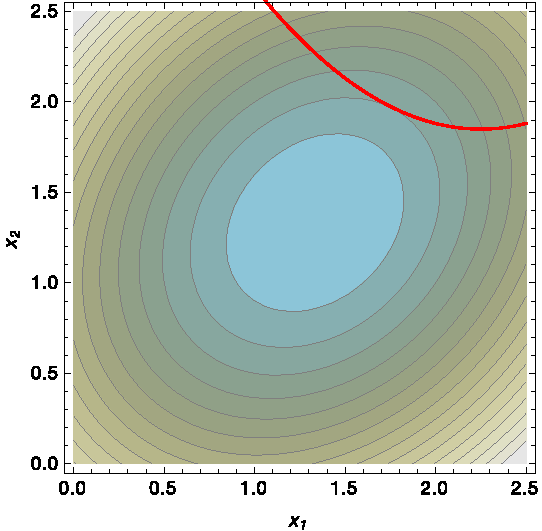
\includegraphics[width=4in]{opt_fig}
  \end{center}
  \caption{A contour plot of the function $f_0 (x_1,x_2) = (x_1 - 1)^2 + (x_2 - 1)^2 - x_1 x_2 /2$ whose minimum occurs at $(4/3,4/3)$ (i.e., the center of the blue ellipse).  The red line indicates the inequality constraint $f_1 (x_1,x_2)= 1.85 + (x_1 - 2.25)^2 / 2 - x_2 \leq 0$. The picture shows that the constrained minimum occurs at the intersection of the contour tangent line and the active constraint line.}
\end{figure}

The geometric picture implied by Theorem~\ref{theorem:KKT} is that of a game where one would like to decrease the objective $f_0 (\vecnot{x}^*)$ by choosing $\vecnot{y}$ such that $\vecnot{y}^H \nabla f_0 (\vecnot{x}^*) < 0$ but there are  constraints on the set of allowable $\vecnot{y}$'s.
Let $H = \Span ( \{ \nabla h_j (\vecnot{x}^*) \})$ be the subspace of directions that violate the equality constraints at $\vecnot{x}^*$.
Similarly, let the cone of directions that violate the active inequality constraints is given by
\[ F = \left\{ \sum_{i\in A} \lambda_i \nabla f_i (\vecnot{x}^*) \, \middle| \, \lambda_i \geq 0, i \in A   \right\}. \]
Thus, one can only pick directions $\vecnot{y}$ that are orthogonal to all vectors in $H$ and also have a non-positive inner product with all vectors in $F$.

Let the matrix $P$ define the orthogonal projection of $\mathbb{R}^n$ onto $H^\perp$.
Using this, we can translate the equation~\eqref{eq:KKT1} into the statement
\[ -P \nabla f_0 (\vecnot{x}^*) \in P F \]  or ``the projection of the descent direction lies in the projection of the cone of directions that violate the inequality constraints''.
The reason for this is that we can absorb the $\nabla h_j$ terms into the $\nabla f_i$ terms by defining
\[ \vecnot{f}^{(i)} = \nabla f_i (\vecnot{x}^*) + \sum_{j=1}^p \nu_{j,i} \nabla h_j (\vecnot{x}^*) = P \nabla f_i (\vecnot{x}^*) \]
so that $\vecnot{f}^{(i)} \in H^{\perp}$ for $i=0,1,\ldots,m$.
Then, the cone $PF$ is defined by
\[ PF = \left\{ \sum_{i\in A} \lambda_i \vecnot{f}^{(i)} \, \middle| \, \lambda_i \geq 0, i\in A \right\}. \]

If $-P \nabla f_0 (\vecnot{x}^*) \notin P F$, then we project $-P \nabla f_0 (\vecnot{x}^*)$ onto $PF$ to get a non-zero residual $\vecnot{y}$.
The resulting vector gives a direction where the objective function decreases and the constraints remain \emph{almost} satisfied.
The challenge in making this proof precise is that, unless the equality constraints are affine, they may not be exactly satisfied for $t>0$.
In standard proofs of this result, this difficulty is overcome by using the implicit function theorem to construct an $\vecnot{x} (t)$ that starts in the direction of $\vecnot{y}$ but is perturbed slightly to remain feasible.

\begin{proof}
For simplicity, we prove only the case where $h_j (\vecnot{x}) = \vecnot{a}_j^H \vecnot{x} - \vecnot{b}$ is affine and $PF$ does contain a line (i.e., $\{\alpha \vecnot{z}\,|\, \alpha \in \mathbb{R}\}$ for some $\vecnot{z}$).  First, we define 
\[ \vecnot{y} (\vecnot{\lambda},\vecnot{\nu}) = -\nabla f_0 (\vecnot{x}^*) - \sum_{i=1}^m \lambda_i \nabla f_i (\vecnot{x}^*) - \sum_{j=1}^p \nu_j \underbrace{\nabla h_j (\vecnot{x}^*)}_{\vecnot{a}_j}. \]
The vector $\vecnot{y} (\vecnot{\lambda},\vecnot{\nu})$ can be seen as the residual of the descent direction for the objective function after the constraint gradients have been used to cancel some parts.
Next, we let $\vecnot{\nu}^* (\vecnot{\lambda}) = \arg \min_{\vecnot{\nu}\in \mathbb{R}^p} \| \vecnot{y} (\vecnot{\lambda},\vecnot{\nu}) \|_2$
and apply the best approximation theorem to see that
\[ \vecnot{y} (\vecnot{\lambda},\vecnot{\nu}^* (\vecnot{\lambda})) = P \vecnot{y} (\vecnot{\lambda},\vecnot{\nu}), \]
where $P$ is orthogonal projection onto $H^\perp$ and $H = \Span ( \{ \vecnot{a}_j \} )$.
This ensures that each $h_j ( \vecnot{x}^* + t \vecnot{y} (\vecnot{\lambda},\vecnot{\nu}^* (\vecnot{\lambda})) )=0$ for all $\vecnot{\lambda}\in \mathbb{R}^m$ and $t\in \mathbb{R}$.

Continuing, we define $\vecnot{y}^* = \arg \min_{\vecnot{\lambda} \in \mathbb{R}^m, \vecnot{\lambda} \geq \vecnot{0}} \| \vecnot{y} (\vecnot{\lambda},\vecnot{\nu}^* (\vecnot{\lambda})) \|_2 $.
This implies that $\vecnot{y}^*$ is the error vector for the projection of $-P\nabla f_0 (\vecnot{x}^*)$ onto the convex set $PF$.
The projection itself is given by $\vecnot{z}=-P\nabla f_0 - \vecnot{y}^*$ and Lemma~\ref{lemma:convex_proj_lt0} shows that $\left( \vecnot{y}^* \right)^H \left( \vecnot{z} \right) \geq 0$.
Using this, we see that
\[ \left( \vecnot{y}^* \right)^H \left(-P \nabla f_0 (\vecnot{x}^*) \right)
= \left(\vecnot{y}^* \right)^H \left(\vecnot{z}+\vecnot{y}^* \right)
 \geq \| \vecnot{y}^* \|_2^2.
\]
If~\eqref{eq:KKT1} cannot be satisfied by some $\vecnot{\lambda} \geq \vecnot{0}$ and $\vecnot{\nu}$, then $\vecnot{y}^* \neq \vecnot{0}$ and $\| \vecnot{y}^* \|_2 > 0$.
This shows that $\vecnot{y}^*$ points in a direction that decreases the value of the objective function.

But, the $\vecnot{y}^*$ direction is only guaranteed to preserve feasibility to first order (i.e., $(\vecnot{y}^*)^H P \nabla f_i (\vecnot{x}^*) \leq 0$).
To fix this, one can add to $\vecnot{y}^*$ a sufficiently small vector $\vecnot{w}$ satisfying $\vecnot{w}^H P \nabla f_i (\vecnot{x}^*) < 0$ for all $i=1,2,\ldots,m$.
Such a $\vecnot{w}$ lies in the ``interior of the polar cone of $PF$'' and will exist as long as $PF$ does not contain a line.
With this modification, the definition of the derivative implies that, for sufficiently small $t$, $\vecnot{x}(t) = \vecnot{x}^* + t (\vecnot{y}^* + \vecnot{w})$ will be a feasible vector satisfying $f_0 (\vecnot{x}(t)) < f_0 (\vecnot{x}^*)$.
\end{proof}

\subsection{Lagrangian Duality}


\begin{definition}
The \defn{optimization}{Lagrangian dual} function is defined to be
\[ g(\vecnot{\lambda},\vecnot{\nu}) \triangleq \inf_{\vecnot{x}\in \mathcal{D}} L(\vecnot{x},\vecnot{\lambda},\vecnot{\nu}). \]
\end{definition}


\begin{lemma}
The Lagrangian dual problem
\begin{align*}
\mathrm{maximize} \quad & g(\vecnot{\lambda},\vecnot{\nu}) \\
\mathrm{subject\,to} \quad & \vecnot{\lambda} \geq 0
\end{align*}
has a unique maximum value $d^* \leq p^*$.
This property is known as \defn{optimization}{weak duality}.
\end{lemma}

\begin{proof}
The Lagrangian dual function is concave because it is the pointwise infimum of affine functions
\begin{align*}
g(\alpha\vecnot{\lambda}+&(1-\alpha)\vecnot{\lambda}',\alpha\vecnot{\nu}+(1-\alpha)\vecnot{\nu}') \\
&= \inf_{\vecnot{x}\in \mathcal{D}} L(\vecnot{x},\alpha\vecnot{\lambda}+(1-\alpha)\vecnot{\lambda}',\alpha\vecnot{\nu}+(1-\alpha) \vecnot{\nu}') \\
&= \inf_{\vecnot{x}\in \mathcal{D}} \big( \alpha L(\vecnot{x},\vecnot{\lambda},\vecnot{\nu}) + (1-\alpha) L(\vecnot{x},\vecnot{\lambda}',\vecnot{\nu}') \big) \\
&\geq \inf_{\vecnot{x}\in \mathcal{D}} \alpha L(\vecnot{x},\vecnot{\lambda},\vecnot{\nu}) + \inf_{\vecnot{x}'\in \mathcal{D}} (1-\alpha) L(\vecnot{x}',\vecnot{\lambda}',\vecnot{\nu}') \\
&= \alpha g(\vecnot{\lambda},\vecnot{\nu}) + (1-\alpha) g(\vecnot{\lambda}',\vecnot{\nu}').
\end{align*}
Thus, it follows from Theorem~\ref{theorem:convex_unique_min}) that it has a unique maximum value $d^*$ which can be upper bounded by
\begin{align*}
g(\vecnot{\lambda},\vecnot{\nu})
&= \inf_{\vecnot{x}\in \mathcal{D}} L(\vecnot{x},\vecnot{\lambda},\vecnot{\nu})
\stackrel{(a)}{\leq} \inf_{\vecnot{x}\in \mathcal{F}} L(\vecnot{x},\vecnot{\lambda},\vecnot{\nu}) \\
&\stackrel{(b)}{=} p^* + \sum_{i=1}^m \lambda_i f_i (\vecnot{x})
\stackrel{(c)}{\leq} p^*,
\end{align*}
where $(a)$ is implied by $\mathcal{F} \subseteq \mathcal{D}$, $(b)$ follows from $h_j(\vecnot{x}) = 0$ for $\vecnot{x}\in \mathcal{F}$, and $(c)$ holds by combining $f_i(\vecnot{x}) \leq 0$ for $\vecnot{x}\in \mathcal{F}$ and $\lambda_i \geq 0$.
\end{proof}

The Lagrangian dual function can be $-\infty$ for a wide range of $(\vecnot{\lambda},\vecnot{\nu})$.
In this case, it makes sense to eliminate these points by defining the implicit constraint set
\begin{align*}
\mathcal{C} &\triangleq \left\{ (\vecnot{\lambda},\vecnot{\nu}) \in \mathbb{R}^m \times \mathbb{R}^p | \vecnot{\lambda}\succeq \vecnot{0},  g(\vecnot{\lambda},\vecnot{\nu}) > -\infty \right\}.
\end{align*}
The points $(\vecnot{\lambda},\vecnot{\nu}) \in \mathcal{C}$ are called \textbf{dual feasible}.

\begin{definition}
If $d^* = p^*$, then one says that \defn{optimization}{strong duality} holds for the problem.
\end{definition}

\begin{theorem}
If strong duality holds for an optimization problem, then the KKT conditions are sufficient for optimality? 
\end{theorem}
\begin{proof}
If x,u,v satisfy KKT, then 
\end{proof}

\begin{example}
For the first LP in Definition~\ref{def:standard_lp}, the Lagrangian is given by
\[ L(\vecnot{x},\vecnot{\lambda},\vecnot{\nu}) = \vecnot{c}^T \vecnot{x} + \vecnot{\nu}^T (A\vecnot{x}-\vecnot{b}) - \vecnot{\lambda}^T \vecnot{x}, \]
where the $\vecnot{\lambda}$ term is negative because the constraint is $\lambda \succeq \vecnot{0}$.
Thus, the Lagrangian dual function is given by
\begin{equation*}
g(\vecnot{\lambda},\vecnot{\nu})
= \inf_{\vecnot{x}\in \mathcal{D}} L(\vecnot{x},\vecnot{\lambda},\vecnot{\nu})
= \begin{cases} -\vecnot{b}^T \vecnot{\nu} & \text{if }A^T \vecnot{\nu} - \vecnot{\lambda} + \vecnot{c} = \vecnot{0} \\
-\infty & \text{otherwise}. \end{cases}
\end{equation*}
Solving the implicit constraint and using the fact that $\vecnot{\lambda} \succeq \vecnot{0}$, one gets the dual LP problem
\begin{align*}
\mathrm{maximize} \quad & -\vecnot{b}^T \vecnot{\nu} \\
\mathrm{subject\,to} \quad & A^T \vecnot{\nu} + c \succeq \vecnot{0}.
\end{align*}
Strong duality for linear programs says that, if the original LP has an optimal solution (i.e., it is neither unbounded nor infeasible), then the dual LP has an optimal solution of the same value.
\end{example}

\subsection{Convex Optimization}

\begin{definition} \label{def:convex_opt}
An optimization problem in standard form is called \defn{optimization}{convex} if the function $f_i$ is convex for $i=0,1,\ldots,m$, the function $h_j$ is affine (i.e., $h_j(\vecnot{x}) = \vecnot{a}_j^T \vecnot{x} - b_j)$ for $j=1,2,\ldots,p$, and $\mathcal{D}=\RealNumbers^n$. 
\end{definition}

\begin{problem}
For a convex standard-form optimization problem (i.e.,  satisfying Definition~\ref{def:convex_opt}), show that the feasible set is a convex set.
\end{problem}

Applying Theorem~\ref{theorem:convex_unique_min} to this setup shows that a convex standard-form optimization problem has a unique minimum value.
Also, if the function $f_0$ is strictly convex, then the minimum value achieved uniquely.
There are a number of stronger conditions that also imply strong duality for convex optimization problems.
\defn{optimization}{Slater's condition} is stated below as a theorem and its proof can be found in~\cite[Sec.~5.3.2]{Boyd-2004}.
 
\begin{theorem}[Slater's Condition]
If a convex optimization problem has a point $\vecnot{x}_0$ where $f_i(\vecnot{x}_0) < 0$ for $i=1,\ldots,m$ and $h_j (\vecnot{x}_0) = 0$ for $j=1,\ldots,p$, then strong duality holds for the problem.
\end{theorem}


\begin{example}
For a channel with colored noise, the input distribution that maximizes the achievable information rate can be found by solving the convex optimization problem, known as water-filling, given by
\begin{align*}
\mathrm{minimize} \quad & -\sum_{i=1}^n \log \left( x_i + \alpha_i \right) \\
\mathrm{subject\,to} \quad & \sum_{i=1}^n x_i = P \\
& \vecnot{x} \succeq 0.
\end{align*}
Choosing $x_i = \frac{P}{n}$ for $i=1,\ldots,n$ gives a point that satisfies Slater's condition, so strong duality holds for this problem.
\end{example}

\begin{example}
For the water-filling problem, the Lagrangian can be written as
\[ L(\vecnot{x},\vecnot{\lambda},\nu) = - \sum_{i=1}^n \log(x_i + \alpha_i) - \sum_{i=1}^m \lambda_i x_i + \nu \left( -P + \sum_{i=1}^n x_i \right)  \]
and the Lagrangian dual is given by $g(\vecnot{\lambda},\nu)
= \inf_{\vecnot{x}\in \mathbb{R}^n} L(\vecnot{x},\vecnot{\lambda},\nu)$.

If $\lambda_i <0$, then the Lagrangian tends to $-\infty$ as $x_i \to -\infty$.
Thus, the system is implicitly constrained to have $\lambda_i \geq 0$.
The first-order optimality conditions, for $i=1,2,\ldots,n$, are given by
\[ -\frac{1}{x_i + \alpha_i} - \lambda_i + \nu = 0.
\]
Solving this for $x_i$ shows that $x_i$ is increasing in $\lambda _i$ (for $\lambda_i \geq 0$) and this implies that $g(\vecnot{\lambda},\nu)$ is decreasing in $\lambda_i$ (for $\lambda_i \geq 0$ and $x_i \geq 0$).

Thus, the expression
$\max_{\vecnot{\lambda} \geq 0} g(\vecnot{\lambda},\nu)$
is given by choosing the smallest non-negative $\lambda_i$'s for which $x_i \geq 0$.
This implies that
\[ (x_i,\lambda_i) = \begin{cases} \left( \frac{1}{\nu} - \alpha _i, 0 \right) & \text{if }\nu < \frac{1}{\alpha_i} \\ \left(0,\nu-\frac{1}{\alpha_i}\right) & \text{if } \nu \geq \frac{1}{\alpha_i}. \end{cases} \]
From this, the value of $\nu$ can be determined by solving
\[\sum_{i=1}^n x_i = \sum_{i=1}^n \max \left\{ 0,\frac{1}{\nu}-\alpha_i \right\} = P. \]
By strong duality, the optimal value of the dual problem equals the optimal value of the original problem.
Finally, the problem can be easily solved for a range of $P$ values by sweeping through a range of $\nu$ values and computing $P$ in terms of $\nu$.
\end{example}
